\section{Methods \label{sec:rank_lists_fusion}}

The idea of rank lists' fusion is to combine multiple rank lists in such a way that the resulting rank list produced is a more accurate modelling of a perfect rank list.
A perfect rank list contain every true links (same author document pairs) at the top and every false links (different author document pair) at the bottom, therefore maximizing every metrics in Section~\ref{sec:rl_eval}.

One proposed method is based on the Z-Score normalization, and the second one use the logistic regression.

\subsection{Z-Score Fusion}

When merging rank lists, the following problem arise: Due to the difference of distance metric and/or text representation, the scores used in the different rank lists are of different order of magnitude.
Thus, simply applying the arithmetic mean on the scores for each rank list is not effective.

To mitigate this problem, a simple and rather effective approach is to normalize the scores of each rank lists independently using the Z-Score (See Definition~\ref{def:z_score} in Section~\ref{sec:normalization}).
Then one can compute a resulting score for each link as the arithmetic mean of scores in every Z-Score normalized rank lists.
The rank list can then be sorted by this new score.

Additionally, this method provide a framework for the fusion with both distance metrics and similarity metrics.
If distances and similarity score are encountered for a fusion, flipping the score sign for either the distance rank lists or similarity rank lists before or after the Z-Score normalization allow to fix these metrics differences.

Even though this method lack theoretical foundations, it can provide good results and does not have any parameters.

Example~\ref{ex:z_score_fusion} exemplify the Z-Score fusion computation using two simple rank lists.

\begin{example}
  \caption{A two rank lists Z-Score fusion}
  \label{ex:z_score_fusion}

  \begin{subexample}{\linewidth}
    \centering
    \subcaption{Rank list A (Mean = 50, Std = 40.82)}
    \begin{tabular}{c l r r}
      \toprule
      Rank & Link & Score & Z-Score \\
      \midrule
      1st & (0, 2) & $0$ & $-1.22$ \\
      2nd & (1, 2) & $50$ & $0$ \\
      3rd & (0, 1) & $100$ & $1.22$ \\
      \bottomrule
    \end{tabular}
  \end{subexample}

  \vspace{0.5cm}

  In this example, for the sake of simplicity, the scores does not satisfy the triangle inequality.

  \vspace{0.5cm}

  \begin{subexample}{\linewidth}
    \centering
    \subcaption{Rank list B (Mean = 0.33, Std = 0.17)}
    \begin{tabular}{c l r r}
      \toprule
      Rank & Link & Score & Z-Score \\
      \midrule
      1st & (0, 2) & $0.1$ & $-1.37$ \\
      2nd & (0, 1) & $0.4$ & $0.39$ \\
      3rd & (1, 2) & $0.5$ & $0.98$ \\
      \bottomrule
    \end{tabular}
  \end{subexample}

  \vspace{0.5cm}

  \begin{subexample}{\linewidth}
    \centering
    \subcaption{Z-Score fusion}
    \begin{tabular}{c l r}
      \toprule
      Rank & Link & Mean Z-Score \\
      \midrule
      1st & (0, 2) & $(-1.22 + (-1.37)) / 2$ = $-1.30$ \\
      2nd & (1, 2) & $(0 + 0.98) / 2$ = $0.49$ \\
      3rd & (0, 1) & $(0.39 + 1.22) / 2$ = $0.81$ \\
      \bottomrule
    \end{tabular}
  \end{subexample}

\end{example}

\subsection{Regression Fusion \label{sec:regression_fusion}}

This second fusion method is based on logistic regression and is called regression fusion in this study.

Each rank list is ordered by a score, this score depends on the distance measure and text representation used, thus the order of magnitude across rank list can be different.
To avoid this problem, the second solution is to express the scores into a probability of being a true link.
To do so, the logistic regression is used.
This method is similar to the one proposed in \textit{Le Calvé and Savoy (2000)}'s paper~\cite{le_calve_database_merging} and was used to merge rank list issued from information retrieval systems.

The idea is to learn a logistic regression model for each combination of text representation and distance metrics (here denoted \textit{type of rank list}).
From each distinct rank list, features for each link are created.
The features are: the log of the relative rank and the link score.
Since a probability of being a true link is desired, the target value (labels) for each link is either $1.00$ for the true links or $0.00$ when it is a false link.
This feature construction is the same as the one used for the regression-based clustering method (ref. Section~\ref{sec:regression_based_clustering}).

One model per type of rank list is trained.
This model can provide, for any new same type rank lists, true link probabilities for each link.

The probability framework can now be used on the rank lists.
To obtain the most reliable probability given multiple observations (different rank lists), the regression fusion consists in computing the expected value of each link's probability using these observations.
In this case, the final value for sorting the rank list is an arithmetic mean of the probabilities, since no weighting is used on the rank lists.

The main advantage of this methodology is that it uses concrete statistical concepts.
But this technique has one main issue: it requires training samples to train the model.

\subsection{Veto}

To try to further improve the results, the idea here is to provide a veto power for the rank lists.

The following assumption is made:
If a link have a low probability in a rank list before the fusion, it probably indicates a false link, thus having this link at the bottom of the rank list after the fusion should improve the results.

To fulfil this assumption an introduce a veto, we used to following algorithm:

\begin{enumerate}
  \item In every rank lists before the fusion, find every links where the probability is under a certain threshold.
  \item Alter their probabilities (probability of being a true link) with $-\infty$.
  \item Perform the regression fusion (by averaging the probabilities)
\end{enumerate}

No matter the rank list, every links below the probability threshold will have its final score also equal to $-\infty$ since the average with any number and $-\infty$ is always $-\infty$.
When sorting the rank list, the links with a resulting $-\infty$ score will subsequently be ranked at the bottom.
This first veto method is called $-\infty$-veto in this study.

Example~\ref{ex:veto_ninf} showcase when the veto can provide better results than the standard fusion in Example~\ref{ex:noveto}.
In the example, rank list $1$ gives a $0.20$ true link probability for a link with $ID = 4$, but rank list $3$ give this link a $0.80$ true link probability.
The link with $ID = 3$ is ranked $3$rd, but with the veto the link is ranked $5$th.

One problem arise with this solution, multiple links can have a $-\infty$ probability.
They thus can not be sorted anymore.
False positives (true links affected by the veto), will thus be ranked randomly at the bottom.

The proposed solution is to set the probability of the affected links to one of these values instead: $0$, $-1$ or $-n$, with $n$ equal to the number of rank lists to fuse.
The greater, the value, the stronger the penalty for the affected links if they are under the threshold for multiple rank lists.
The $-\infty$ method is the only real veto, in the first meaning of the veto definition, the other methods can be considered as a weighted veto.

The $-n$, method provide a way to avoid having tie and keep the strong impact of the $-\infty$-veto when a lot of rank list are fused.
For example, if $9$ rank lists are fused.
By setting any link score to $-9$ will ensure that even if every other rank lists this link have a true link probability of $1.00$, the probability is lower than $0.00$, the lowest probability obtainable by regression fusion.

By setting to $0$, $-1$ or $-n$, it lightens the veto effect and conserve an order for the bottom rank links.
Example~\ref{ex:veto_0} show the $0$-veto strategy.
Here the link with $ID = 4$ is ranked $4$th due to a lighter effect of this veto.
Link with $ID = 5$ is still rank at the bottom.

\begin{example}
  \centering
  \caption{Fusion without veto}
  \label{ex:noveto}

  \begin{subexample}{\linewidth}
    \centering
    \subcaption{Rank lists}
    \resizebox{\linewidth}{!}{
    \begin{tabular}{c c|c c|c c}
      \toprule
      \multicolumn{2}{c}{Rank list 1} &
      \multicolumn{2}{c}{Rank list 2} &
      \multicolumn{2}{c}{Rank list 3} \\
      Link ID & Score &
      Link ID & Score &
      Link ID & Score \\
      \midrule
      0 & 0.95 & 0 & 0.90 & 5 & 0.90 \\
      1 & 0.75 & 3 & 0.70 & 4 & 0.80 \\
      2 & 0.60 & 4 & 0.65 & 0 & 0.70 \\
      3 & 0.50 & 1 & 0.50 & 1 & 0.60 \\
      4 & 0.20 & 2 & 0.30 & 2 & 0.50 \\
      5 & 0.10 & 5 & 0.10 & 3 & 0.40 \\
      \bottomrule
    \end{tabular}
    }
  \end{subexample}

  \vspace{0.5cm}

  \begin{subexample}{\linewidth}
    \centering
    \subcaption{Rank lists' fusion}
    \resizebox{\linewidth}{!}{
    \begin{tabular}{l l l}
      \toprule
      Rank & Link ID & Average \\
      \midrule
      1st & 0 & $(0.95 + 0.90 + 0.70)/3 = 0.85$ \\
      2nd & 1 & $(0.75 + 0.50 + 0.60)/3 = 0.62$ \\
      3rd & 4 & $(0.20 + 0.65 + 0.80)/3 = 0.55$ \\
      4th & 3 & $(0.50 + 0.70 + 0.40)/3 = 0.53$ \\
      5th & 2 & $(0.60 + 0.30 + 0.50)/3 = 0.47$ \\
      6th & 5 & $(0.10 + 0.10 + 0.90)/3 = 0.37$ \\
      \bottomrule
    \end{tabular}
    }
  \end{subexample}
\end{example}

\begin{example}
  \centering
  \caption{Fusion with $-\infty$-veto at 0.25}
  \label{ex:veto_ninf}

  \begin{subexample}{\linewidth}
    \centering
    \subcaption{Rank lists}
    \resizebox{\linewidth}{!}{
    \begin{tabular}{c c|c c|c c}
      \toprule
      \multicolumn{2}{c}{Rank list 1} &
      \multicolumn{2}{c}{Rank list 2} &
      \multicolumn{2}{c}{Rank list 3} \\
      Link ID & Score &
      Link ID & Score &
      Link ID & Score \\
      \midrule
      0 & 0.95 & 0 & 0.90 & 5 & 0.90 \\
      1 & 0.75 & 3 & 0.70 & 4 & 0.80 \\
      2 & 0.60 & 4 & 0.65 & 0 & 0.70 \\
      3 & 0.50 & 1 & 0.50 & 1 & 0.60 \\
      4 & -inf & 2 & 0.30 & 2 & 0.50 \\
      5 & -inf & 5 & -inf & 3 & 0.40 \\
      \bottomrule
    \end{tabular}
    }
  \end{subexample}

  \vspace{0.5cm}

  \begin{subexample}{\linewidth}
    \centering
    \subcaption{Rank lists' fusion}
    \resizebox{\linewidth}{!}{
    \begin{tabular}{l l l}
      \toprule
      Rank & Link ID & Average \\
      \midrule
      1st & 0 & $(0.95 + 0.90 + 0.70)/3 = 0.85$ \\
      2nd & 1 & $(0.75 + 0.50 + 0.60)/3 = 0.62$ \\
      3rd & 3 & $(0.50 + 0.70 + 0.40)/3 = 0.53$ \\
      4th & 2 & $(0.60 + 0.30 + 0.50)/3 = 0.47$ \\
      5-6th & 4 & $(-\infty + 0.65 + 0.80)/3 = -\infty$ \\
      5-6th & 5 & $(-\infty + -\infty + 0.90)/3 = -\infty$ \\
      \bottomrule
    \end{tabular}
    }
  \end{subexample}
\end{example}

\begin{example}
  \centering
  \caption{Fusion with $0$-veto at 0.25}
  \label{ex:veto_0}

  \begin{subexample}{\linewidth}
    \centering
    \subcaption{Rank lists}
    \resizebox{\linewidth}{!}{
    \begin{tabular}{c c|c c|c c}
      \toprule
      \multicolumn{2}{c}{Rank list 1} &
      \multicolumn{2}{c}{Rank list 2} &
      \multicolumn{2}{c}{Rank list 3} \\
      Link ID & Score &
      Link ID & Score &
      Link ID & Score \\
      \midrule
      0 & 0.95 & 0 & 0.90 & 5 & 0.90 \\
      1 & 0.75 & 3 & 0.70 & 4 & 0.80 \\
      2 & 0.60 & 4 & 0.65 & 0 & 0.70 \\
      3 & 0.50 & 1 & 0.50 & 1 & 0.60 \\
      4 & 0.00 & 2 & 0.30 & 2 & 0.50 \\
      5 & 0.00 & 5 & 0.00 & 3 & 0.40 \\
      \bottomrule
    \end{tabular}
    }
  \end{subexample}

  \vspace{0.5cm}

  \begin{subexample}{\linewidth}
    \centering
    \subcaption{Rank lists' fusion}
    \resizebox{\linewidth}{!}{
    \begin{tabular}{l l l}
      \toprule
      Rank & Link ID & Average \\
      \midrule
      1st & 0 & $(0.95 + 0.90 + 0.70)/3 = 0.85$ \\
      2nd & 1 & $(0.75 + 0.50 + 0.60)/3 = 0.62$ \\
      3rd & 3 & $(0.50 + 0.70 + 0.40)/3 = 0.53$ \\
      4th & 4 & $(0.00 + 0.65 + 0.80)/3 = 0.48$ \\
      5th & 2 & $(0.60 + 0.30 + 0.50)/3 = 0.47$ \\
      6th & 5 & $(0.00 + 0.00 + 0.90)/3 = 0.30$ \\
      \bottomrule
    \end{tabular}
    }
  \end{subexample}
\end{example}

\subsection{Soft-veto}

As an extension to the veto method, an additional desired constraint is to favor top ranked link and as well as penalizing bottom ranked links.

In any rank list, top ranked links should correspond to documents with the same author, and bottom ranked links should correspond to documents with different authors.
Assuming that the top ranks are true links after the rank lists' fusion, these links should also appear top ranked.
The same reasoning can be applied for the bottom links by assuming them as false links.
A weighting curve can be design accordingly.
The idea of this curve is to boost the score of top ranked links and hindered the score of bottom ranked links before the fusion.

First, the scores' distribution must be understood.
By observing the graph score/distance over rank, Figure~\ref{fig:distance_over_rank}, we can clearly observe the top rank links and bottom rank links have a sharper difference in distance than the ones in the middle section.

Using the inverse of the sigmoid function, a weighting curve satisfying our constraints can be modelled.
The choice on the sigmoid function was arbitrary.
Any function in form of an \textit{S} can be used.
The hyperbolic tangent or the arc tangent function could also be possible.

Definition~\ref{def:sigmoid} show the sigmoid function and its inverse function.

\begin{definition}[Sigmoid and Sigmoid inverse function \label{def:sigmoid}]
  Sigmoid:
  \begin{gather*}
    S(x) = \frac{1}{1+e^{-x}}
  \end{gather*}

  Sigmoid inverse:
  \begin{gather*}
    S^{-1}(x) = -\ln{\frac{x-1}{x}}
  \end{gather*}
\end{definition}

Since the sigmoid inverse function is continuous and the number of links in a rank list is discrete, the idea is to sample values in this curve at regular intervals.
Also, since the sigmoid function is defined from $-\infty$ to $+\infty$ and the rank list have a finite size, an interval must be select.

This interval directly control the steepness of the curve and thus influence the strength of the veto.
To control the steepness, a parameter called $c$ is introduced.
$c$ correspond to a position on the x-axis of the sigmoid function.
The sampling of the sigmoid inverse is done in the interval $\left[S(c), S(c)\right]$.
A large interval gives a greater steepness and a small interval a less steep curve.
$c$ can not be equal to 0 otherwise the interval consist of a single number (also known as degenerate interval).
The $c$ parameter must be in the interval $\left]0, \infty\right[$.
With a value close to $0$, the soft-veto have a weak effect.
With a large value, for example 20, the soft veto has a strong effect on the top and bottom, see Figure~\ref{fig:s_curve_c}.

To break the curve symmetry and to be able to increase the conservation of the top rank while decreasing the conservation of the bottom ranked.
The solution proposed is to have a new parameter $r$.
$r \cdot N$ samples are taken for the left side of the curve $\left[S(-c), S(0)\right]$
And $(1-r) \cdot N$ samples for the right side of the curve $\left[S(0), S(c)\right]$.
Figure~\ref{fig:s_curve_r} shows the $r$ parameter influence on a sigmoid with $c = 4$ and $r \in \left[0.1, 0.9\right]$.
The $r$ parameter must be in the interval $\left]0, 1\right[$.
With a value close to $0$ the soft-veto have a strong effect on the top ranked links.
With a large value, a strong effect on the bottom ranked links, see Figure~\ref{fig:s_curve_r}.

To apply the soft-veto, each score in the rank list is multiplied by the curve at the corresponding rank.
This soft-veto methodology aimed to be used on rank list before fusing, to have a more cleaved decision on the links positions.
This strategy can be use on any type of scoring method (similarity, distances, Z-Score scores or probabilities).

\begin{figure}
  \centering
  \caption{Distance values over rank in the rank list using the smoothed Manhattan distance, $500$-MF tokens on the Brunet dataset}
  \label{fig:distance_over_rank}
  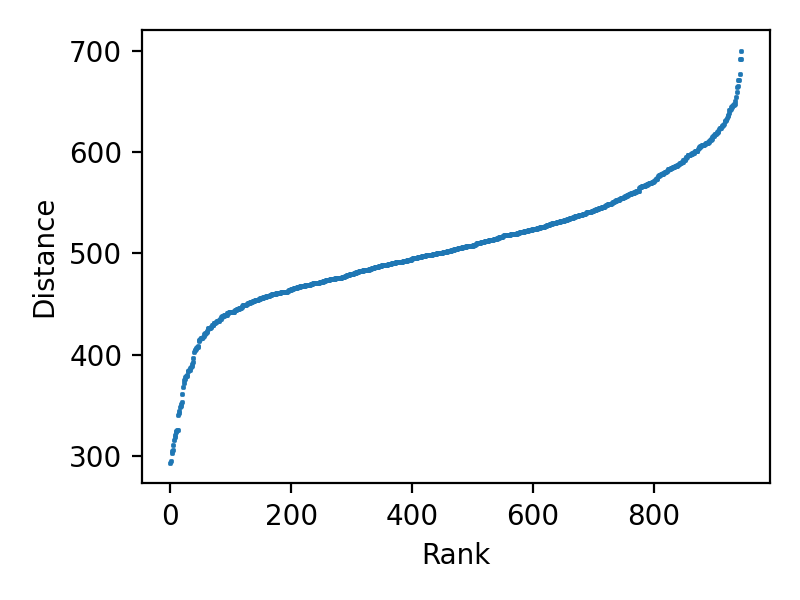
\includegraphics[width=\linewidth]{img/distance_over_rank.png}
\end{figure}

\begin{figure}
  \centering
  \caption{Soft-veto curve parameters}
  \label{fig:s_curve_params}

  \subcaption{$S^-1(x)$, 1000 samples (for a rank list with 1000 links) in $\left[S(-c), S(+c)\right]$}
  \label{fig:s_curve_c}
  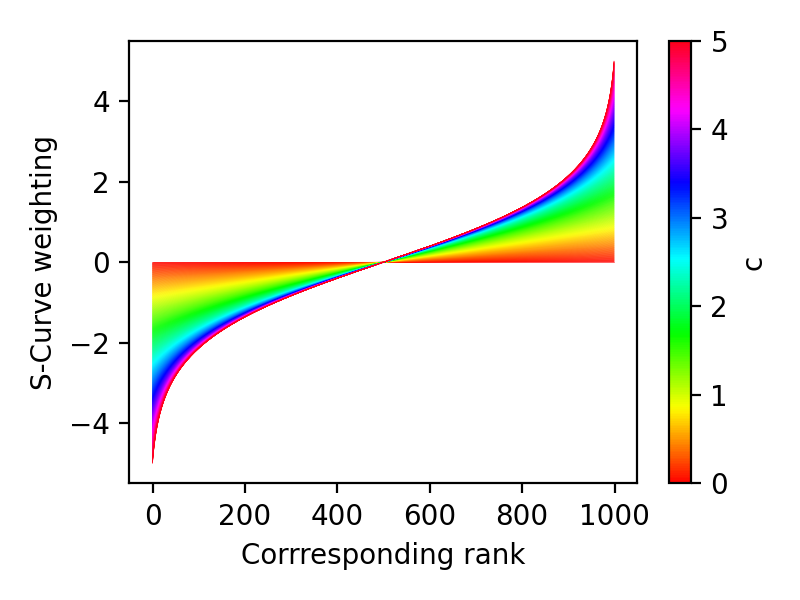
\includegraphics[width=\linewidth]{img/s_curve_c.png}

  \vspace{0.5cm}

  \subcaption{1000 sample of $S^-1(x)$ with $r \cdot N$ samples for $\left[S(-c), S(0)\right]$ and $(1-r) \cdot N$ samples for $\left[S(0), S(c)\right]$}
  \label{fig:s_curve_r}
  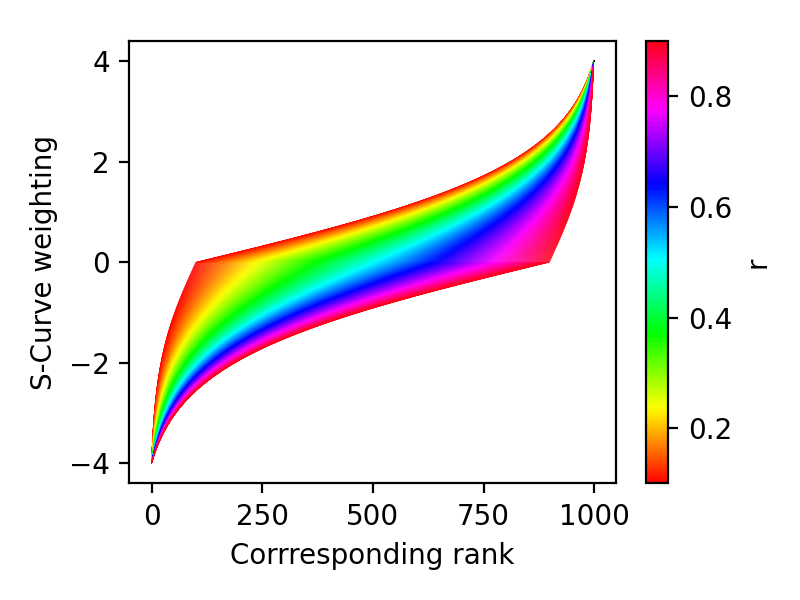
\includegraphics[width=\linewidth]{img/s_curve_r.png}

  \vspace{0.5cm}

  \subcaption{Example of a curve with $c=4$ and $r=0.85$}
  \label{fig:s_curve_example}
  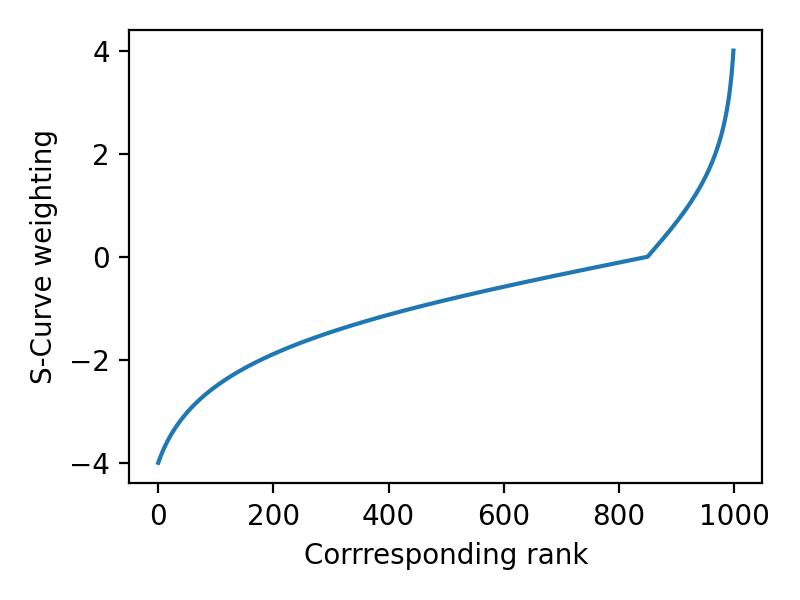
\includegraphics[width=0.9\linewidth]{img/s_curve_example.png}
\end{figure}
